\documentclass[12pt,a4paper,]{report}
\usepackage{lmodern}


% Overwrite \begin{figure}[htbp] with \begin{figure}[H]
\usepackage{float}
\let\origfigure=\figure
\let\endorigfigure=\endfigure
\renewenvironment{figure}[1][]{%
\origfigure[H]
}{%
\endorigfigure
}

% fix for pandoc 1.14
\providecommand{\tightlist}{%
  \setlength{\itemsep}{0pt}\setlength{\parskip}{0pt}}

% TP: hack to truncate list of figures/tables.
\usepackage{truncate}
\usepackage{caption}
\usepackage{tocloft}
% TP: end hack

\usepackage{amssymb,amsmath}
\usepackage{ifxetex,ifluatex}

% Only use fixltx2e if using pre-2015 kernels
\begingroup\expandafter\expandafter\expandafter\endgroup
\expandafter\ifx\csname IncludeInRelease\endcsname\relax
  \usepackage{fixltx2e}
\fi

\ifnum 0\ifxetex 1\fi\ifluatex 1\fi=0 % if pdftex
  \usepackage[T1]{fontenc}
  \usepackage[utf8]{inputenc}
\mathbf{
\else % if luatex or xelatex
  \ifxetex
    \usepackage{mathspec}
    \usepackage{xltxtra,xunicode}
  \else
    \usepackage{fontspec}
  \fi
  \defaultfontfeatures{Mapping=tex-text,Scale=MatchLowercase}
  \newcommand{\euro}{€}
\fi
% use upquote if available, for straight quotes in verbatim environments
\IfFileExists{upquote.sty}{\usepackage{upquote}}{}
% use microtype if available
\IfFileExists{microtype.sty}{%
\usepackage{microtype}
\UseMicrotypeSet[protrusion]{basicmath} % disable protrusion for tt fonts
}{}
\usepackage{longtable,booktabs}
\usepackage{graphicx}
\makeatletter
\def\maxwidth{\ifdim\Gin@nat@width>\linewidth\linewidth\else\Gin@nat@width\fi}
\def\maxheight{\ifdim\Gin@nat@height>\textheight\textheight\else\Gin@nat@height\fi}
\makeatother
% Scale images if necessary, so that they will not overflow the page
% margins by default, and it is still possible to overwrite the defaults
% using explicit options in \includegraphics[width, height, ...]{}
\setkeys{Gin}{width=\maxwidth,height=\maxheight,keepaspectratio}
\ifxetex
  \usepackage[setpagesize=false, % page size defined by xetex
              unicode=false, % unicode breaks when used with xetex
              xetex]{hyperref}
\else
  \usepackage[unicode=true]{hyperref}
\fi
\hypersetup{breaklinks=true,
            bookmarks=true,
            pdfauthor={Angel-Emilio Villegas Sanchez},
            pdftitle={A Heuristics-Based Approach to the Prediction of FODs in Fermi-Lowdin Orbital Self Interaction Correction (FLOSIC) Theory},
            colorlinks=true,
            citecolor=blue,
            urlcolor=blue,
            linkcolor=magenta,
            pdfborder={0 0 0}}
\urlstyle{same}  % don't use monospace font for urls
\setlength{\parindent}{0pt}
\setlength{\parskip}{6pt plus 2pt minus 1pt}
\setlength{\emergencystretch}{3em}  % prevent overfull lines
\setcounter{secnumdepth}{5}

% 



% Table of contents formatting
\renewcommand{\contentsname}{Table of Contents}
\setcounter{tocdepth}{3}

% Headers and page numbering
\usepackage{fancyhdr}
\pagestyle{fancy}
\fancyhf{}
\fancyfoot[C]{\thepage}
\renewcommand{\headrulewidth}{0pt}
% Following package is used to add background image to front page
\usepackage{wallpaper}

% Table package
\usepackage{ctable}% http://ctan.org/pkg/ctable

% Deal with 'LaTeX Error: Too many unprocessed floats.'
\usepackage{morefloats}
% or use \extrafloats{100}
% add some \clearpage

% % Chapter header
% \usepackage{titlesec, blindtext, color}
% \definecolor{gray75}{gray}{0.75}
% \newcommand{\hsp}{\hspace{20pt}}
% \titleformat{\chapter}[hang]{\Huge\bfseries}{\thechapter\hsp\textcolor{gray75}{|}\hsp}{0pt}{\Huge\bfseries}

% % Fonts and typesetting
% \setmainfont[Scale=1.1]{Helvetica}
% \setsansfont[Scale=1.1]{Verdana}

% FONTS
\usepackage{xunicode}
\usepackage{xltxtra}
\defaultfontfeatures{Mapping=tex-text} % converts LaTeX specials (``quotes'' --- dashes etc.) to unicode
% \setromanfont[Scale=1.01,Ligatures={Common},Numbers={OldStyle}]{Palatino}
% \setromanfont[Scale=1.01,Ligatures={Common},Numbers={OldStyle}]{Adobe Caslon Pro}
%Following line controls size of code chunks
% \setmonofont[Scale=0.9]{Monaco}
%Following line controls size of figure legends
% \setsansfont[Scale=1.2]{Optima Regular}

% CODE BLOCKS
\usepackage[utf8]{inputenc}
\usepackage{listings}
\usepackage{color}
%Addtional Packages
\usepackage[ruled, vlined]{algorithm2e}
\setlength{\algomargin}{1em}

% JAVA CODE BLOCKS
%\definecolor{backcolour}{RGB}{242,242,242}
%\definecolor{javared}{rgb}{0.6,0,0}
%\definecolor{javagreen}{rgb}{0.25,0.5,0.35}
%\definecolor{javapurple}{rgb}{0.5,0,0.35}
%\definecolor{javadocblue}{rgb}{0.25,0.35,0.75}

\lstdefinestyle{javaCodeStyle}{
  language=Java,                         % the language of the code
  backgroundcolor=\color{backcolour},    % choose the background color; you must add \usepackage{color} or \usepackage{xcolor}
  basicstyle=\fontsize{10}{8}\sffamily,
  breakatwhitespace=false,
  breaklines=true,
  keywordstyle=\color{javapurple}\bfseries,
  stringstyle=\color{javared},
  commentstyle=\color{javagreen},
  morecomment=[s][\color{javadocblue}]{/**}{*/},
  captionpos=t,                          % sets the caption-position to bottom
  frame=single,                          % adds a frame around the code
  numbers=left,
  numbersep=10pt,                         % margin between number and code block
  keepspaces=true,                       % keeps spaces in text, useful for keeping indentation of code (possibly needs columns=flexible)
  columns=fullflexible,
  showspaces=false,                      % show spaces everywhere adding particular underscores; it overrides 'showstringspaces'
  showstringspaces=false,                % underline spaces within strings only
  showtabs=false,                        % show tabs within strings adding particular underscores
  tabsize=2                              % sets default tabsize to 2 spaces
}

%Attempt to set math size
%First size must match the text size in the document or command will not work
%\DeclareMathSizes{display size}{text size}{script size}{scriptscript size}.
%\DeclareMathSizes{12}{13}{7}{7}

% ---- CUSTOM AMPERSAND
% \newcommand{\amper}{{\fontspec[Scale=.95]{Adobe Caslon Pro}\selectfont\itshape\&}}

% HEADINGS
\usepackage{sectsty}
\usepackage[normalem]{ulem}
\sectionfont{\bfseries\centering} %Centered, Bold
\subsectionfont{\bfseries\raggedright} % Bold
\subsubsectionfont{\bfseries\itshape} %Bold Italic
\paragraphfont{\bfseries\raggedright}
% \sectionfont{\rmfamily\mdseries\Large}
% \subsectionfont{\rmfamily\mdseries\scshape\normalsize}
% \subsubsectionfont{\rmfamily\bfseries\upshape\normalsize}

% Set figure legends and captions to be smaller sized sans serif font
\usepackage[font={footnotesize,sf}]{caption}

\usepackage{siunitx}

% Adjust spacing between lines to 1.5
\usepackage{setspace}
% \onehalfspacing
\doublespacing
\raggedbottom

% Set margins
\usepackage[top=1in,bottom=1in,left=1in,right=1in]{geometry}
\setlength\parindent{0.5in} % indent at start of paragraphs (set to 0.3?)
\setlength{\parskip}{9pt}
\usepackage{indentfirst}

% Add space between pararaphs
% http://texblog.org/2012/11/07/correctly-typesetting-paragraphs-in-latex/
% \usepackage{parskip}
% \setlength{\parskip}{\baselineskip}

% Set colour of links to black so that they don't show up when printed
\usepackage{hyperref}
\hypersetup{colorlinks=false, linkcolor=black}

% Tables
\usepackage{booktabs}
\usepackage{threeparttable}
\usepackage{array}
\usepackage{makecell}
\newcolumntype{x}[1]{%
>{\centering\arraybackslash}m{#1}}%

% Allow for long captions and float captions on opposite page of figures
% \usepackage[rightFloats, CaptionBefore]{fltpage}

% Don't let floats cross subsections
% \usepackage[section,subsection]{extraplaceins}

% Rotate images and tables
\usepackage{float}
\usepackage{pdfpages}
\usepackage{pdflscape}
\usepackage{graphicx}
\usepackage{rotating}

% Custom math
\usepackage{bbold}
\DeclareMathOperator*{\argmin}{\arg\!\min}

% pandoc-crossref definitions

% We add the lines below from pandoc-crossref because we are using the --include-in-header flag
% see here: https://lierdakil.github.io/pandoc-crossref/#latex-output-and---include-in-header
% This LaTeX code is obtained by getting pandoc-crossref to dump it
% see here: https://github.com/lierdakil/pandoc-crossref/issues/326

\makeatletter
\@ifpackageloaded{subfig}{}{\usepackage{subfig}}
\@ifpackageloaded{caption}{}{\usepackage{caption}}
\captionsetup[subfloat]{margin=0.5em}
\AtBeginDocument{%
\renewcommand*\figurename{Figure}
\renewcommand*\tablename{Table}
}
\AtBeginDocument{%
\renewcommand*\listfigurename{List of Figures}
\renewcommand*\listtablename{List of Tables}
}
\newcounter{pandoccrossref@subfigures@footnote@counter}
\newenvironment{pandoccrossrefsubfigures}{%
\setcounter{pandoccrossref@subfigures@footnote@counter}{0}
\begin{figure}\centering%
\gdef\global@pandoccrossref@subfigures@footnotes{}%
\DeclareRobustCommand{\footnote}[1]{\footnotemark%
\stepcounter{pandoccrossref@subfigures@footnote@counter}%
\ifx\global@pandoccrossref@subfigures@footnotes\empty%
\gdef\global@pandoccrossref@subfigures@footnotes{{##1}}%
\else%
\g@addto@macro\global@pandoccrossref@subfigures@footnotes{, {##1}}%
\fi}}%
{\end{figure}%
\addtocounter{footnote}{-\value{pandoccrossref@subfigures@footnote@counter}}
\@for\f:=\global@pandoccrossref@subfigures@footnotes\do{\stepcounter{footnote}\footnotetext{\f}}%
\gdef\global@pandoccrossref@subfigures@footnotes{}}
\@ifpackageloaded{float}{}{\usepackage{float}}
\floatstyle{ruled}
\@ifundefined{c@chapter}{\newfloat{codelisting}{h}{lop}}{\newfloat{codelisting}{h}{lop}[chapter]}
\floatname{codelisting}{Listing}
\newcommand*\listoflistings{\listof{codelisting}{List of Listings}}
\makeatother

\begin{document}

\begin{titlepage}
    \begin{center}

    % Delete the following line
    % to remove the UCL header logo
    \ThisULCornerWallPaper{0.1}{style/univ_logo.eps}

        \vspace*{2.5cm}

        \huge
        A Heuristics-Based Approach to the Prediction of FODs in
        Fermi-Lowdin Orbital Self Interaction Correction (FLOSIC) Theory

        

        \vspace{1.5cm}

        \Large
        Angel-Emilio Villegas Sanchez

        \vspace{1.5cm}

        \normalsize
        A thesis presented for the degree of\\
        Master's of Science

        \vfill

        \normalsize
        Supervised by:\\
        Dr.~Juan Ernesto Peralta \\ Dr.~Koblar Alan Jackson

        \vspace{0.8cm}

        % Uncomment the following line
        % to add a centered university logo
        % \includegraphics[width=0.4\textwidth]{style/univ_logo.eps}

        \normalsize
        Central Michigan University\\
        February 2024

        % Except where otherwise noted, content in this thesis is licensed under a Creative Commons Attribution 4.0 License (http://creativecommons.org/licenses/by/4.0), which permits unrestricted use, distribution, and reproduction in any medium, provided the original work is properly cited. Copyright 2015,Tom Pollard.

    \end{center}
\end{titlepage}


% This is where the converted markdown files will go 
\pagenumbering{arabic}

\tableofcontents

\newpage

\chapter{Introduction}\label{introduction}

\section{Density-Functional Theory
(DFT)}\label{density-functional-theory-dft}

\subsection{Hohenberg-Kohn Theorems}\label{hohenberg-kohn-theorems}

\subsection{Kohn-Sham Formulation}\label{kohn-sham-formulation}

\subsection{Limitations of DFT}\label{limitations-of-dft}

\section{The Self-Interaction Error
(SIC)}\label{the-self-interaction-error-sic}

\subsection{Perdew-Zunger SIC}\label{perdew-zunger-sic}

\section{The FLOSIC Method}\label{the-flosic-method}

\subsection{The Fermi-Lowdin Orbital
(FLOs)}\label{the-fermi-lowdin-orbital-flos}

The following transformation of the canonical orbitals is
Equation~\ref{eq:FLO}

\begin{equation}\protect\hypertarget{eq:FLO}{}{F_i(\mathbf{r})=\sum_j^N \frac{\psi_j^*\left(\mathbf{a}_i\right) \psi_j(\mathbf{r})}{\sqrt{n\left(\mathbf{a}_i\right)}}}\label{eq:FLO}\end{equation}

\subsection{The Fermi-Lowdin Orbital Descriptors
(FODs)}\label{the-fermi-lowdin-orbital-descriptors-fods}

\section{The NRLMOL Code}\label{the-nrlmol-code}

\begin{itemize}
\tightlist
\item
  Describe the code and status of usability
\end{itemize}

\subsection{Overview of Code}\label{overview-of-code}

\begin{itemize}
\tightlist
\item
  Big-picture description of how the code works.
\end{itemize}

\subsection{FOD Determination and Practical
Considerations}\label{fod-determination-and-practical-considerations}

\begin{itemize}
\tightlist
\item
  Describe methods used to input FODs into the FLOSIC program.
\item
  Prime motivation behind this project: an automated and faster process
  to begin calculations, informed from ``empirical'' data, capable to
  extending to larger systems.
\end{itemize}

\section{FOD Geometric Motifs}\label{fod-geometric-motifs}

\begin{itemize}
\tightlist
\item
  Describe how FODs arrange themselves similar to LDQ Theory. This
  (emergent?) behavior makes it
\end{itemize}

As noted in paper X, optimized FODs get arranged in geometries similar
to Thompson structures. This regular structure is most apparent in
monoatomic systems, but the reagular FOD arrangement distorts in the
presence of additional atoms.

\subsection{SP3 Arrangements}\label{sp3-arrangements}

\subsection{SP3D Arrangement}\label{sp3d-arrangement}

\subsection{Dominance Schema}\label{dominance-schema}

\begin{itemize}
\tightlist
\item
  Sometimes FODs are closer to atoms that are of lesser atomic number
  \(Z\) than the neighbouring heavier atoms. This could be attributed to
  shielding caused by the filled shells of periods 3 and above. The
  behavior is described in Figure~\ref{fig:dominance}. This will play a
  special part in the prediction of bonding FODs.
\end{itemize}

\begin{figure}
\hypertarget{fig:dominance}{%
\centering
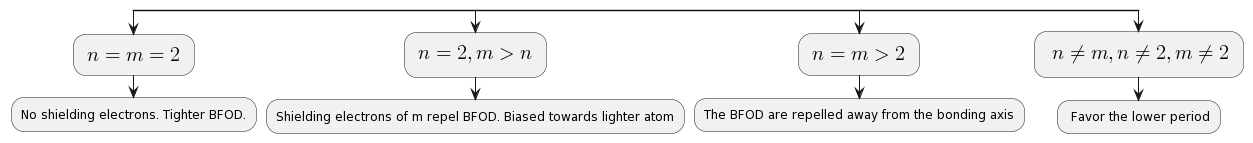
\includegraphics{source/figures/dominance.png}
\caption{dominance}\label{fig:dominance}
}
\end{figure}

\chapter{The FOD-Lego Program}\label{the-fod-lego-program}

\begin{itemize}
\tightlist
\item
  Note: Different name needed probably
\end{itemize}

\section{General Overview}\label{general-overview}

\begin{itemize}
\tightlist
\item
  Give a \textbf{Big-Picture} overview as seen in image
  Figure~\ref{fig:overview}
\end{itemize}

\begin{figure}
\hypertarget{fig:overview}{%
\centering
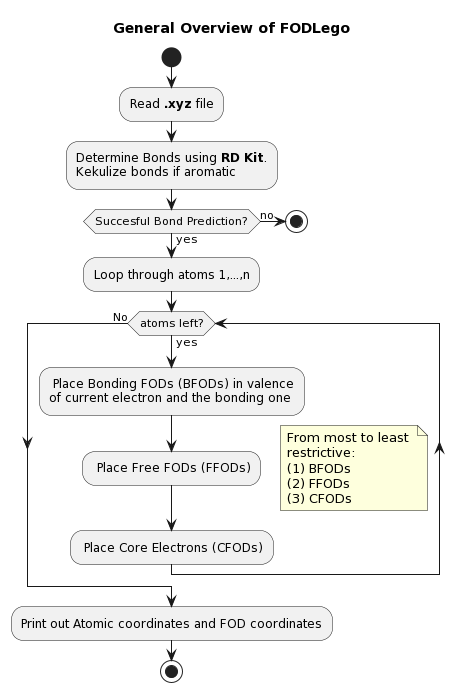
\includegraphics{source/figures/overview.png}
\caption{overview}\label{fig:overview}
}
\end{figure}

\subsection{A Heuristic-Based Approach to FOD
Placement}\label{a-heuristic-based-approach-to-fod-placement}

\begin{itemize}
\tightlist
\item
  How can Heuristics help in computational problems?
\end{itemize}

\subsection{Monoatomic Calculations}\label{monoatomic-calculations}

\begin{itemize}
\tightlist
\item
  Talk about \emph{Dynamic Programming} and how monoatomic geometries
  could be pieced together in modular fashion (Lego-like).
\end{itemize}

\subsection{Reparametrizing the FOD
geometries}\label{reparametrizing-the-fod-geometries}

\begin{itemize}
\tightlist
\item
  sp3 shells stop being perfect tetrahedra and become irregular in the
  presence of other atoms.
\item
  Describe how to parametrize FODs in irregular tetrahedra for the sp3
  shells.
\end{itemize}

\subsection{Implementation Details}\label{implementation-details}

\begin{itemize}
\tightlist
\item
  Describe code structure and use of object-oriented design
\item
  Describe fundamental as seen in Figure~\ref{fig:classdiag}
\end{itemize}

\begin{figure}
\hypertarget{fig:classdiag}{%
\centering
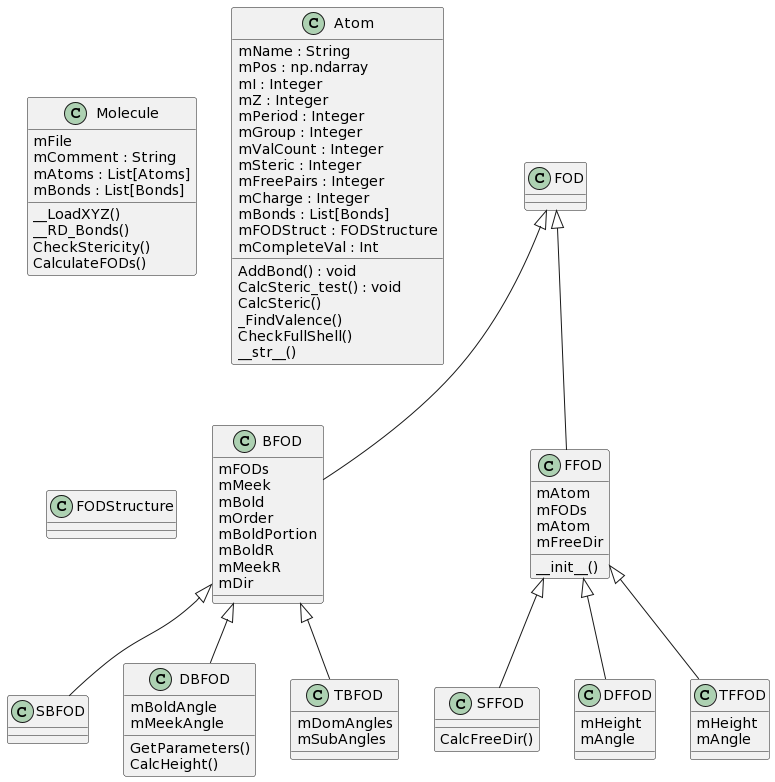
\includegraphics{source/figures/classes.png}
\caption{classes}\label{fig:classdiag}
}
\end{figure}

\section{Determination of FODs}\label{determination-of-fods}

\begin{itemize}
\tightlist
\item
  Describe the different determination heuristics for different types of
  FODs
\end{itemize}

\subsection{Bonding FODs (BFOD)}\label{bonding-fods-bfod}

\subsection{Core FODs (CFOD)}\label{core-fods-cfod}

\subsection{Free FODs (FFOD)}\label{free-fods-ffod}

\begin{itemize}
\tightlist
\item
  Sample Diagram and calculation for Double-FFOD (DFFOD) Heuristic in
  Figure~\ref{fig:sample}. The edge distance is applied to as a
  restriction.
\end{itemize}

\begin{figure}
\hypertarget{fig:sample}{%
\centering
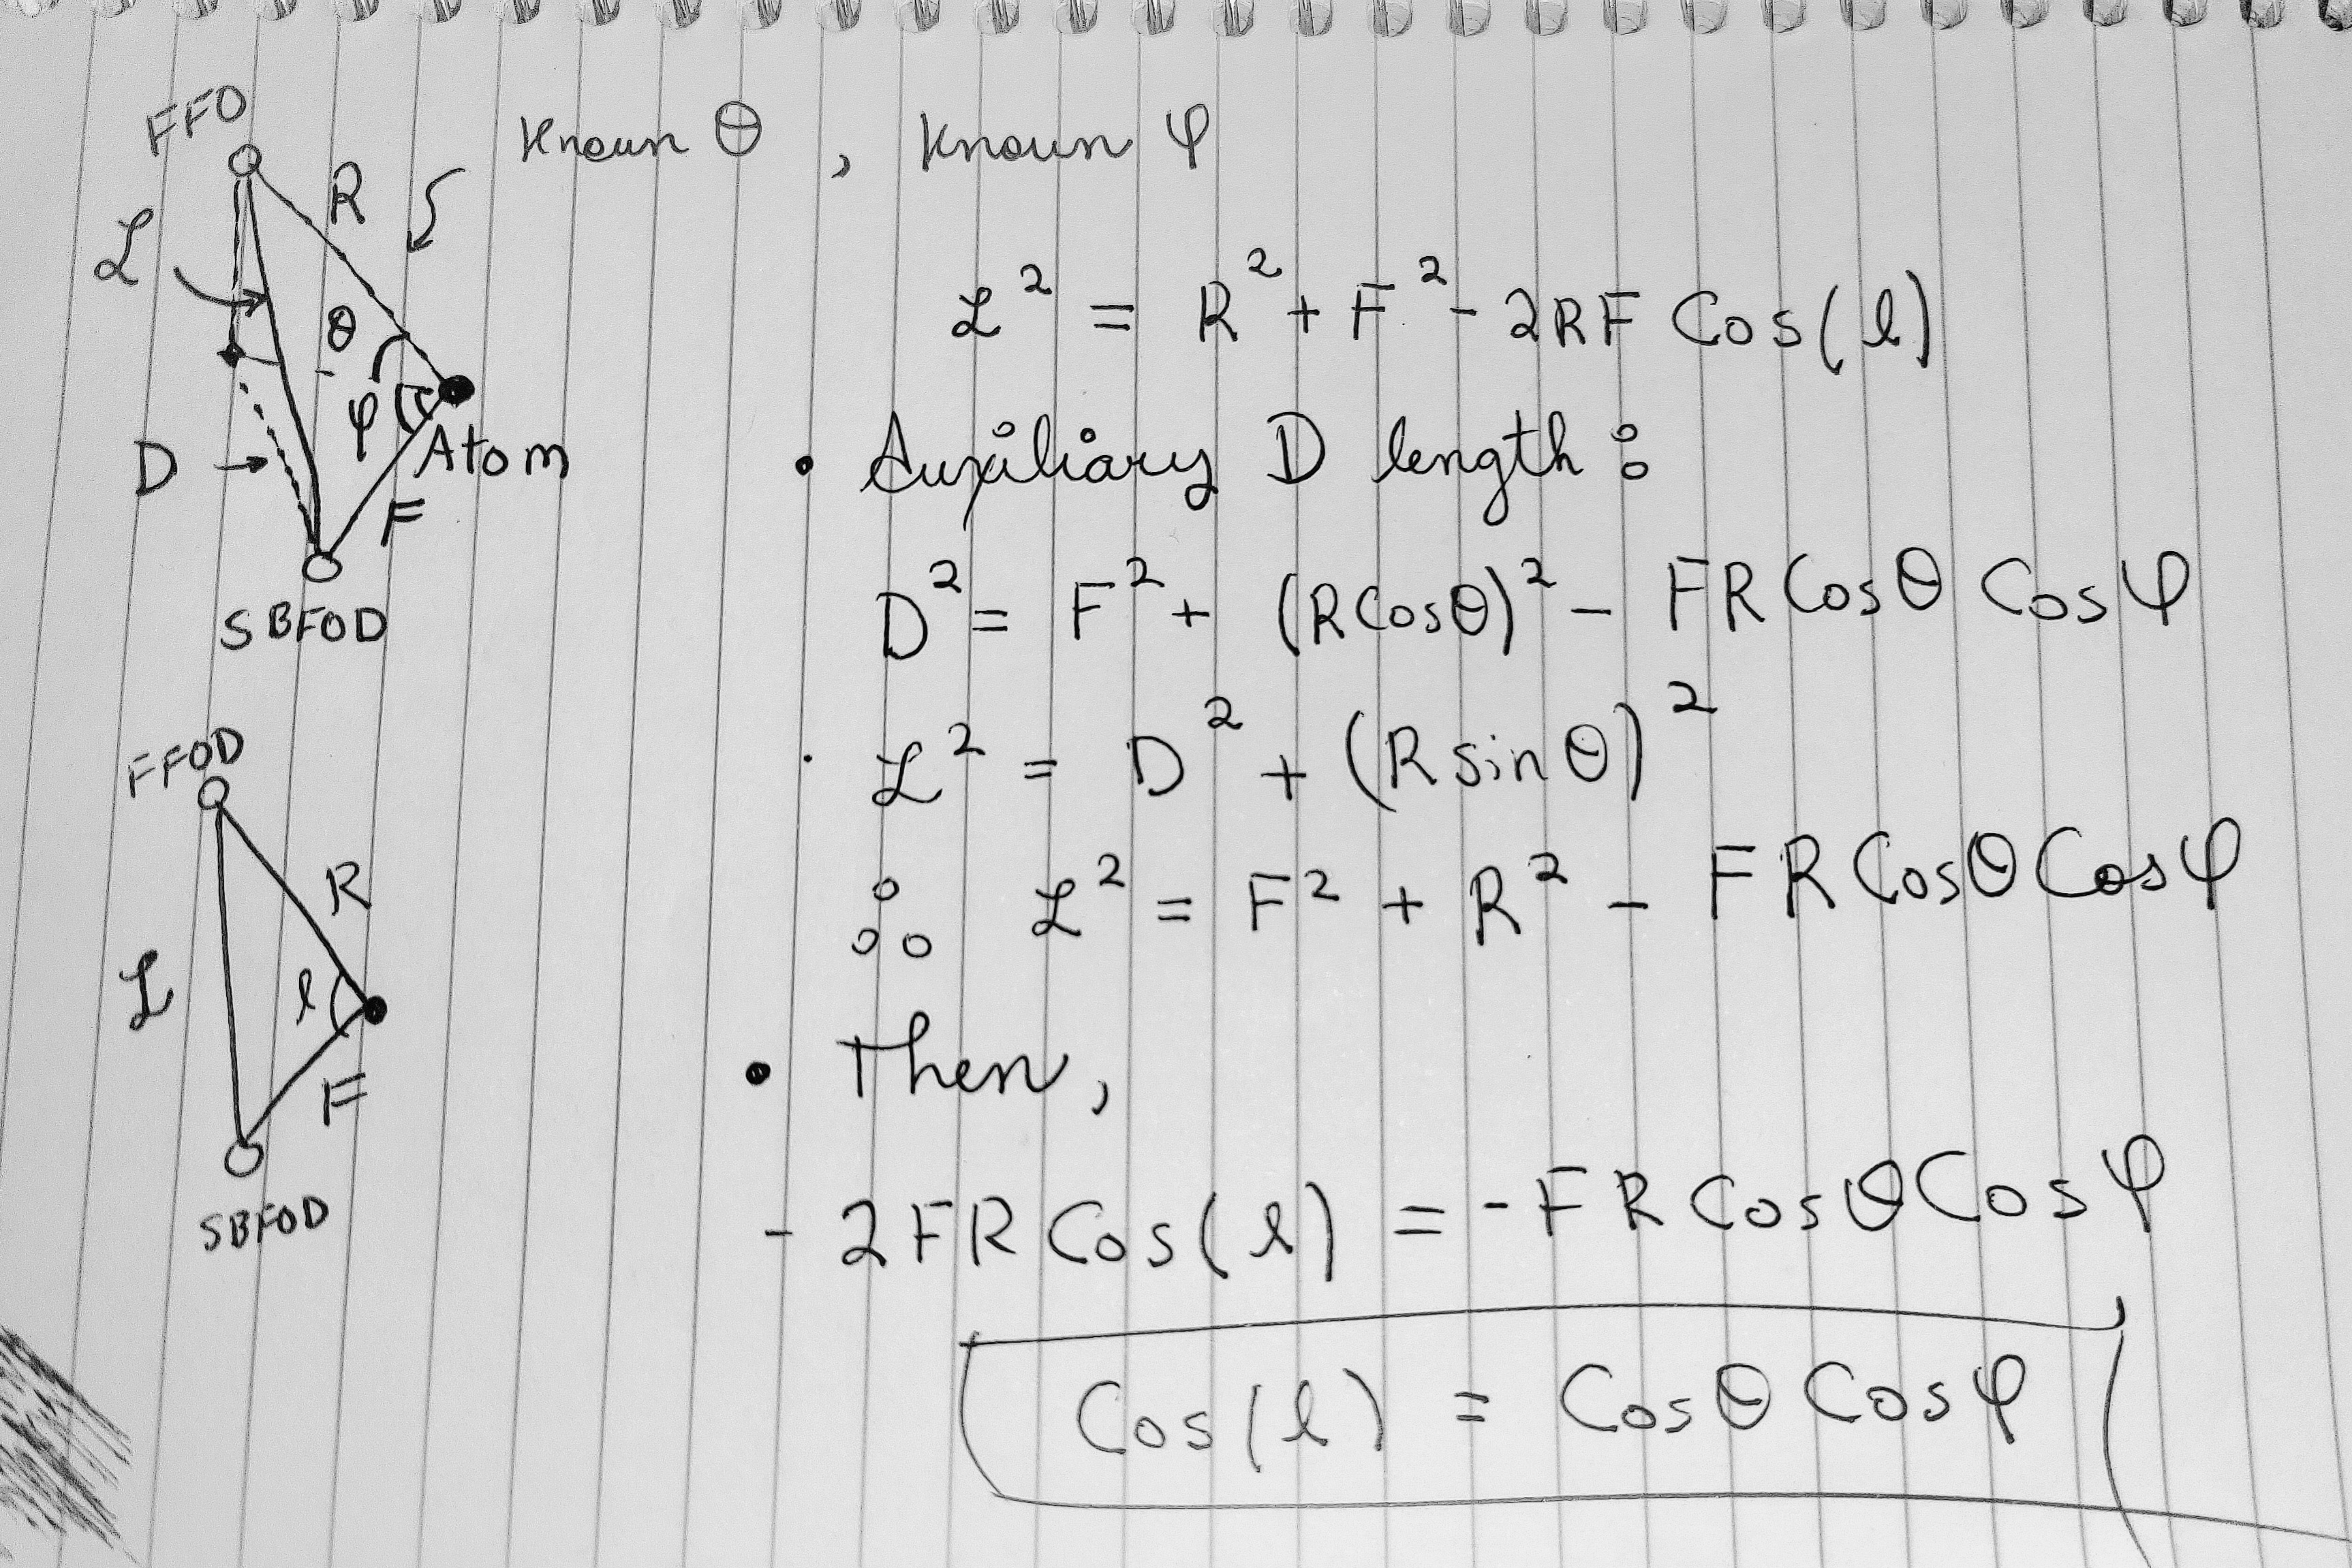
\includegraphics{source/figures/sample.jpg}
\caption{draft DFFOD}\label{fig:sample}
}
\end{figure}

\section{A Data-driven Approach to analyzing
FODs}\label{a-data-driven-approach-to-analyzing-fods}

\subsection{Reverse Determination of
Parameters}\label{reverse-determination-of-parameters}

This is the following implementation used for the reverse determination
of parameters

\begin{algorithm}[H]
 \KwData{ \{$T_n$ | Target FODs\}, \{$P_n$ | Predicted FODs\}}
 \For{$P_n$ in Predicted FODs}{
  Save closest $T_i$ to FOD as $T_{close}$\;
  Initialize a new FOD with $T_{close}$\, $N_n$;
  }
  Reverse Determine parameters for all $N_n$;
 \caption{Reverse Parameter Determination Basic Sequence}
\end{algorithm}

\subsubsection{Free FODs (FFODs)}\label{free-fods-ffods}

The free-direction, described in section XYZ, cannot be determined
exactly. In order to best compare Free FODs in this parameter-based
scheme, I propose using only an average direction formed from the
average of all FFOD vectors and use an evaluation function. A cosine
distance is too flat near its maximum, so a custom function can offer a
more strict metric of our prediction

\begin{equation}\protect\hypertarget{eq:customm}{}{f(\theta) = 1 - \frac{6}{\pi}\theta}\label{eq:customm}\end{equation}

Equation~\ref{eq:customm} yields unity when there at \(0\) degrees
between the vectors, and 0 when there are \(30\) degrees between the
vectors.

\subsection{A database of compiled FOD
Data}\label{a-database-of-compiled-fod-data}

\begin{itemize}
\tightlist
\item
  No current database of FODs. Seeking to create a database
\item
  \textbf{TODO!}

  \begin{itemize}
  \tightlist
  \item
    Design structure of database
  \item
    Using FODLego, then FLOSIC, create optimized structures for a
    selection of molecules (scope?)
  \end{itemize}
\end{itemize}

\chapter{Validity of FOD Prediction}\label{validity-of-fod-prediction}

Explore the predictions done by FODLego

\section{Comparison of Heuristic FODs to FLOSIC-Optimized
FODs}\label{comparison-of-heuristic-fods-to-flosic-optimized-fods}

\begin{itemize}
\tightlist
\item
  \textbf{TODO:}

  \begin{itemize}
  \tightlist
  \item
    Create scatter plots for different parameters described in the
    scheme of previous section.
  \end{itemize}
\end{itemize}

\section{Comparison to FOD-MC}\label{comparison-to-fod-mc}

\section{Biasing Predictions after Sampling
(?)}\label{biasing-predictions-after-sampling}

\begin{itemize}
\item
  \begin{itemize}
  \tightlist
  \item
    Assuming data follows certain trends, we can further modify the
    predictions used in FODLego. For example, the tightening of closed
    shells in heavier atoms in the presence of the next shell closed.
  \end{itemize}
\end{itemize}

\chapter{Discussion/Conclusions}\label{discussionconclusions}

\section{Limitations}\label{limitations}

\subsection{Assumptions}\label{assumptions}

\begin{itemize}
\tightlist
\item
  Explore assumptions such as First neighbors are mainly considered in
  this scheme.
\end{itemize}

\subsection{Automated Bonding
Prediction}\label{automated-bonding-prediction}

\section{For Future Implementation}\label{for-future-implementation}

\subsection{Extending modularity to metal
FODs?}\label{extending-modularity-to-metal-fods}

\begin{itemize}
\tightlist
\item
  Talk about possible parametrization of the \emph{Triaugmented
  Triangular Prism} composed of 9 FODs.
\end{itemize}

\subsection{Spin-Unpolarized
Prediction}\label{spin-unpolarized-prediction}

\end{document}
